\subsection{Zarz�dzanie robotami}
Okienko \texttt{Zarz�dzanie robotami} umo�liwia ustawianie pozycji oraz orientacji wybranego robota na scenie. Zak�adki umo�liwiaj� wyb�r \textit{Pioneera}, kt�rego pozycj� chcemy zmieni�. Aktywne s� tylko zak�adki skojarzone z~robotami dodanymi aktualnie do �wiata. W~polach odpowiedzialnych za pozycj� i~orientacj� robota kolor informuje o~poprawno�ci wprowadzonych danych -- zielony oznacza poprawnie wype�nione pola, natomiast czerwony b��dnie.

\begin{figure}[htbp]
 \centering
 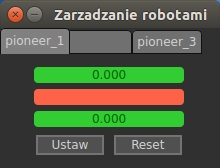
\includegraphics[]{opisy/materialy/zarzadzanie_robotami.jpeg}
 \label{fig:zarzadzanie_robotami}
 \caption{Okno zarz�dzania robotami}
\end{figure}

\subsubsection{Implementacja}
Klasa odpowiadaj�ca za ca�e okienko to \texttt{RobotManagementWindow}. Dziedziczy ona po klasie \texttt{QDialog}. Jej kluczowe metody to:
\begin{lstlisting}[language=C++, numbers=none]
public slots:
	void onAddNewRobot(int id);
	void onHideRobot(int id);
\end{lstlisting}
Odpowiadaj� one za to co dzieje si� w~oknie odpowiednio w~momencie dodania robota i~schowania go. Mianowicie, w~momencie otrzymania odpowiednich sygna��w aktywowana b�d� dezaktywowana jest stosowna zak�adka.

Klasa odpowiadaj�ca za wygl�d zak�adki to \texttt{RobotManagementTab}. Dziedziczy ona po klasie \texttt{QWidget}. Jej kluczowe metody to:
\begin{lstlisting}[language=C++, numbers=none]
void receivedMsg(const boost::shared_ptr<const gazebo::msgs::Int> &msg);
private slots:
	void on_pushButtonUstaw_clicked();
	void on_pushButtonReset_clicked();
\end{lstlisting}













